b\documentclass[12pt]{article}
\usepackage{graphicx}
\graphicspath{ {images/} }
\usepackage[spanish]{babel}
\usepackage[utf8]{inputenc}
\usepackage[backend=biber]{biblatex}
\usepackage[T1]{fontenc}
\usepackage{lmodern}

\begin{document}

\thispagestyle{empty}
\begin{center}
\begin{figure}[h]
\centering

\includegraphics[width=.6\textwidth]{logo.jpg}\\
\end{figure}

\vspace{1cm}
\Large \sc  Instituto Tecnológico y de Estudios Superiores de Monterrey
\\

\vspace{2.5cm}
\Large \bf
\emph{Actividad 1. Conceptos básicos de ciencia de datos}

\vspace{2.5cm}
\Large \bf Nombre del estudiante\\
\vspace{0.3cm}
\Large \bf Matrícula\\
\vspace{3.5cm}
\normalsize \sc \rightline{Ciencia y analítica de datos}
\vspace{0.3cm}
\normalsize \sc \rightline{Fecha}
\end{center}

\newpage

\section{Relación entre los conceptos}
La siguiente figura muestra la relación entre los términos: ciencia de datos (\emph{data science}), aprendizaje automático (\emph{machine learning}) y minería de datos (\emph{data mining}). \\

% Ejemplo de cómo incluir una figura
\begin{figure}[h]
\centering{
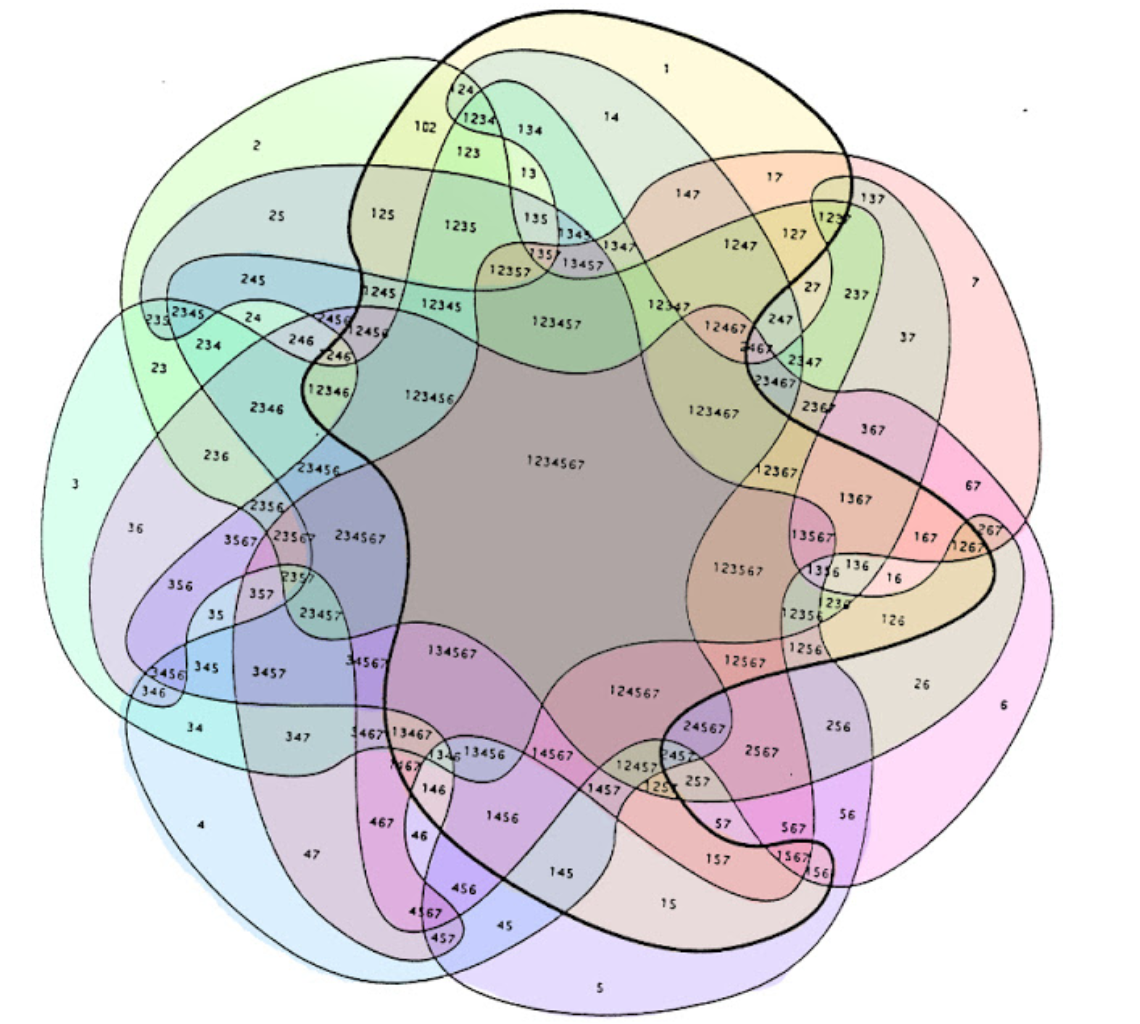
\includegraphics[width=1\textwidth]{imagen.png}\\
\caption{Se debe sustituir por el diagrama gráfico generado}}
\end{figure}

\newpage
\section{Elementos del aprendizaje estadístico}

\begin{itemize}
    \item \textsc{Primer elemento}: Lorem ipsum dolor sit amet, consectetur adipiscing elit, sed do eiusmod tempor incididunt ut labore et dolore magna aliqua. Tristique nulla aliquet enim tortor at auctor. Ipsum dolor sit amet consectetur adipiscing elit. Nunc mattis enim ut tellus. Imperdiet nulla malesuada pellentesque elit. Tortor condimentum lacinia quis vel eros donec ac. Sed faucibus turpis in eu mi bibendum neque. Sed nisi lacus sed viverra tellus in hac habitasse \cite{1}.

    \item \textsc{Segundo elemento}: Lorem ipsum dolor sit amet, consectetur adipiscing elit, sed do eiusmod tempor incididunt ut labore et dolore magna aliqua. Tristique nulla aliquet enim tortor at auctor. Ipsum dolor sit amet consectetur adipiscing elit. Nunc mattis enim ut tellus. Imperdiet nulla malesuada pellentesque elit. Tortor condimentum lacinia quis vel eros donec ac. Sed faucibus turpis in eu mi bibendum neque. Sed nisi lacus sed viverra tellus in hac habitasse \cite{2}.
\end{itemize}

\section{Elementos del aprendizaje automático}

\begin{itemize}
    \item \textsc{Primer elemento}: Lorem ipsum dolor sit amet, consectetur adipiscing elit, sed do eiusmod tempor incididunt ut labore et dolore magna aliqua. Tristique nulla aliquet enim tortor at auctor. Ipsum dolor sit amet consectetur adipiscing elit. Nunc mattis enim ut tellus. Imperdiet nulla malesuada pellentesque elit. Tortor condimentum lacinia quis vel eros donec ac. Sed faucibus turpis in eu mi bibendum neque. Sed nisi lacus sed viverra tellus in hac habitasse \cite{3}. 

    \item \textsc{Segundo elemento}: Lorem ipsum dolor sit amet, consectetur adipiscing elit, sed do eiusmod tempor incididunt ut labore et dolore magna aliqua. Tristique nulla aliquet enim tortor at auctor. Ipsum dolor sit amet consectetur adipiscing elit. Nunc mattis enim ut tellus. Imperdiet nulla malesuada pellentesque elit. Tortor condimentum lacinia quis vel eros donec ac. Sed faucibus turpis in eu mi bibendum neque. Sed nisi lacus sed viverra tellus in hac habitasse \cite{3}. 
\end{itemize}

\newpage
\begin{thebibliography}{a}

% Las referencias a continuación se deben sustituir por las empleadas. Utilice el formato adecuado de los que se muestran a continuación (libro, artículo y/o página web) No cambies el estilo de citación - se ocupa IEEE más común en ingeniería que APA.

% Ejemplo de libro
\bibitem{1}
Michel Goossens, Frank Mittelbach and Alexander Samarin, \emph{The LaTeX Companion}, Addison-Wesley, 1993.

% Ejemplo de artículo
\bibitem{2}
Albert Einstein. \emph{Zur Elektrodynamik bewegter K{\"o}rper}.
\emph{Annalen der Physik}, 322(10):891--921, 1905.

% Ejemplo de página web
\bibitem{3} 
The Data Science Puzzle, Explained. KDnuggets. \\ \url{https://www.kdnuggets.com/2016/03/data-science-puzzle-explained.html} (visitado 04-09-2025)

\end{thebibliography}

\end{document}